\section{Results}\label{sec:results}
\subsection{The evolution}
The cohort ran \gIslands{} islands of \gEvalsIsland{} evaluations each, \gEvalsTotal{} in all, from \gStarted{} to
\gFinished{} UTC, and kept \gElites{} elites, \gTierTwo{} of them at Tier 2. Fig.~\ref{fig:evo} shows the best
score of every island against evaluations, and how the archives filled. The winner came from \gWinIsland, which
started from a best score of \gScoreSobol{} after its Sobol initialisation. Fig.~\ref{fig:lineage} shows that
island's best design at each logged checkpoint, from the same camera.

\begin{figure}[t]
\centering
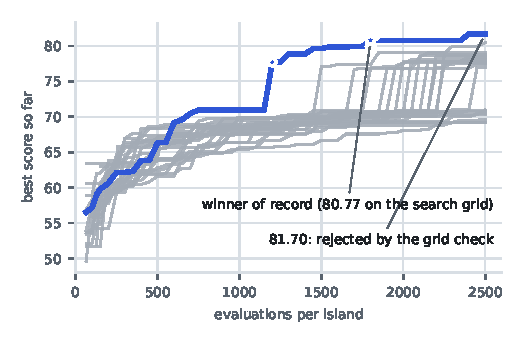
\includegraphics[width=\linewidth]{evolution_best.pdf}\\[2pt]
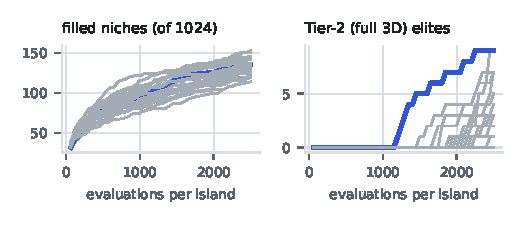
\includegraphics[width=\linewidth]{evolution_archive.pdf}
\caption{Top: best score so far of each island (the winning island in colour; the dot marks its first full-3D
best). Bottom: filled niches and Tier-2 elites per island.}\label{fig:evo}
\end{figure}

\begin{figure*}[t]
\centering
% generated by g3-release-tex: best design of the winning island at each logged checkpoint
\begin{minipage}[t]{0.140\textwidth}\centering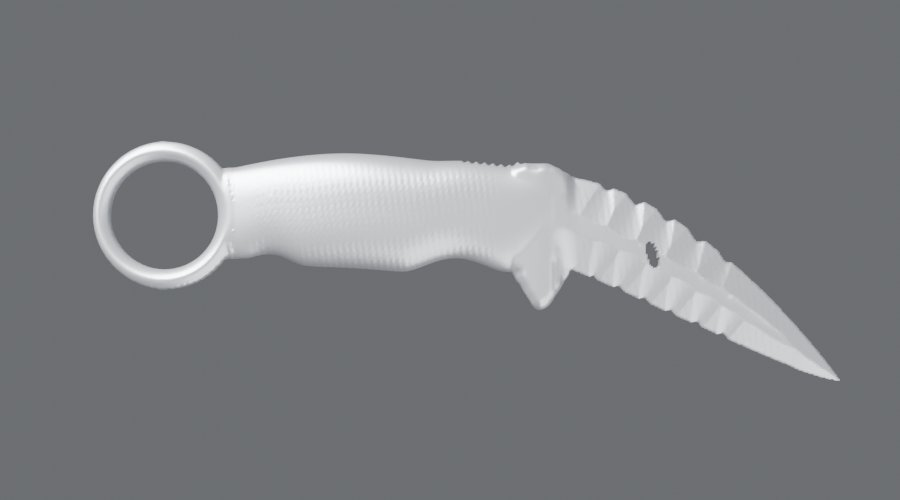
\includegraphics[width=\linewidth]{../../../docs/g3/v3.0.0/img/lineage_00064.jpg}\\[-1pt]{\EItablefont eval 64\\ 56.54, 72.1 g}\end{minipage}\hfill
\begin{minipage}[t]{0.140\textwidth}\centering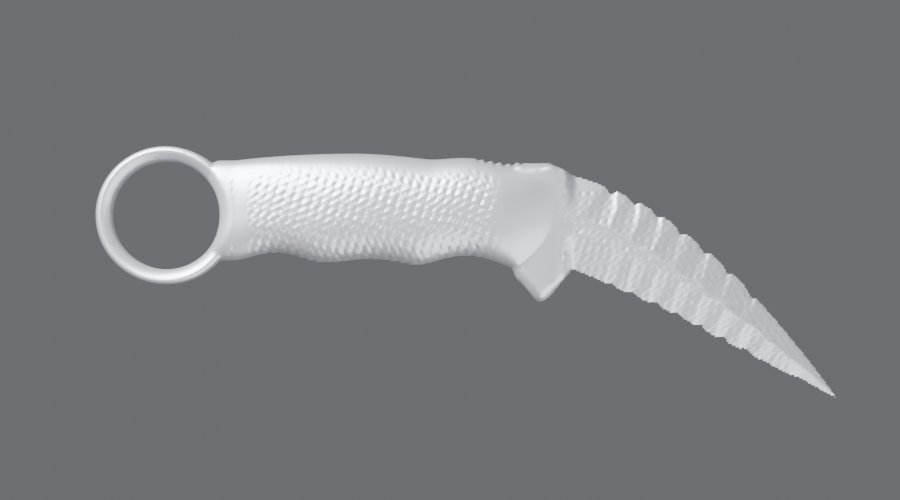
\includegraphics[width=\linewidth]{../../../docs/g3/v3.0.0/img/lineage_00128.jpg}\\[-1pt]{\EItablefont eval 128\\ 59.01, 65.3 g}\end{minipage}\hfill
\begin{minipage}[t]{0.140\textwidth}\centering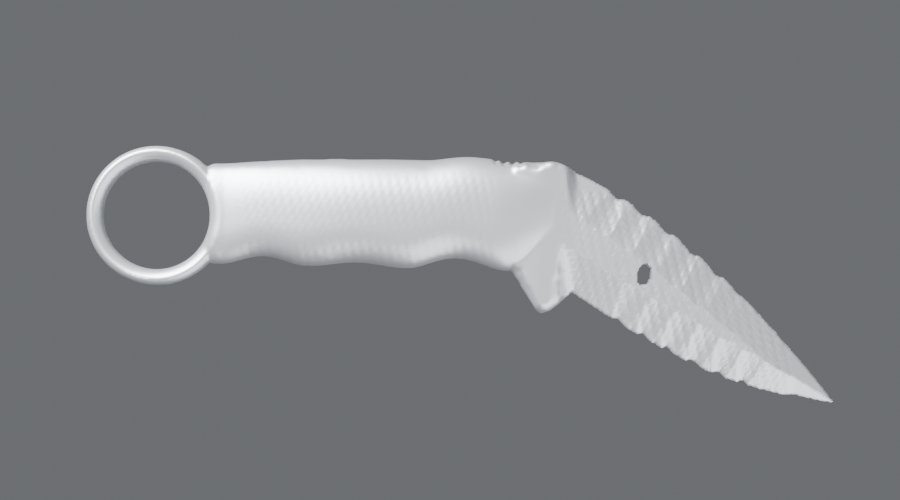
\includegraphics[width=\linewidth]{../../../docs/g3/v3.0.0/img/lineage_00256.jpg}\\[-1pt]{\EItablefont eval 256\\ 62.15, 68.0 g}\end{minipage}\hfill
\begin{minipage}[t]{0.140\textwidth}\centering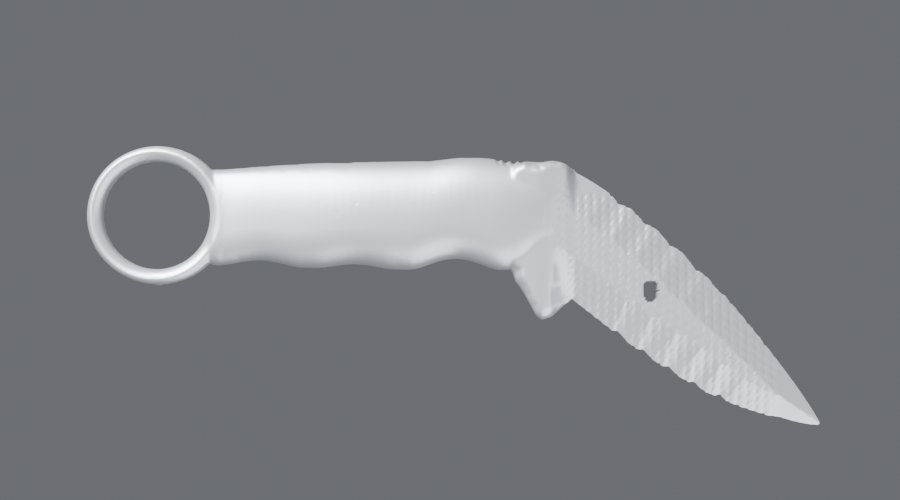
\includegraphics[width=\linewidth]{../../../docs/g3/v3.0.0/img/lineage_00512.jpg}\\[-1pt]{\EItablefont eval 512\\ 66.34, 59.9 g}\end{minipage}\hfill
\begin{minipage}[t]{0.140\textwidth}\centering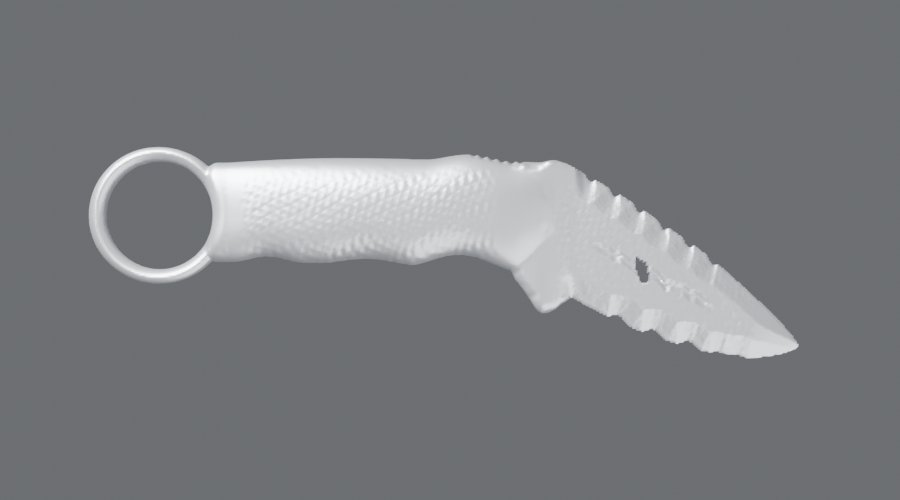
\includegraphics[width=\linewidth]{../../../docs/g3/v3.0.0/img/lineage_01024.jpg}\\[-1pt]{\EItablefont eval 1,024\\ 70.94, 62.4 g}\end{minipage}\hfill
\begin{minipage}[t]{0.140\textwidth}\centering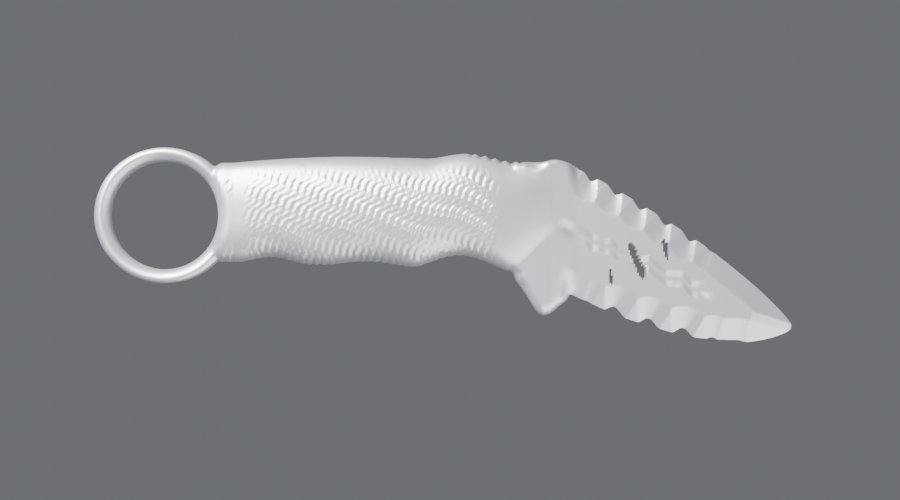
\includegraphics[width=\linewidth]{../../../docs/g3/v3.0.0/img/lineage_02048.jpg}\\[-1pt]{\EItablefont eval 2,048\\ 80.77, 56.0 g\\ \textbf{winner of record}}\end{minipage}\hfill
\begin{minipage}[t]{0.140\textwidth}\centering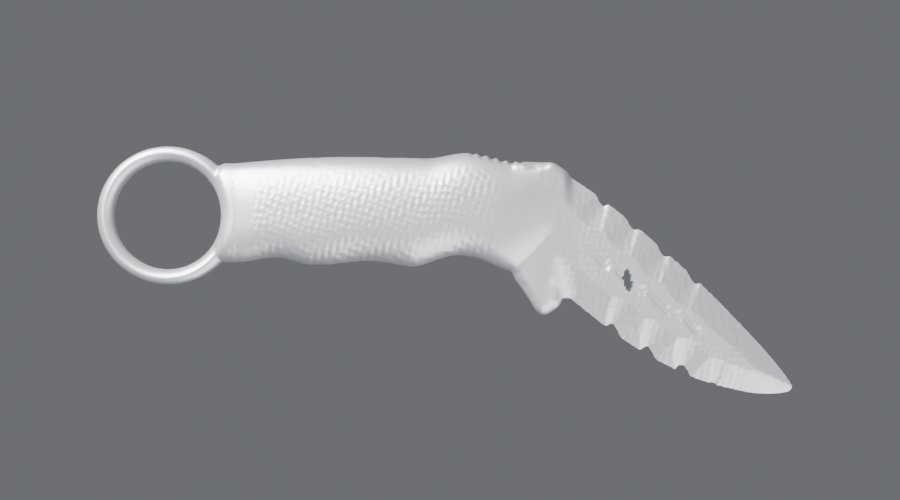
\includegraphics[width=\linewidth]{../../../docs/g3/v3.0.0/img/lineage_02500.jpg}\\[-1pt]{\EItablefont eval 2,500\\ 81.70, 51.3 g\\ \textbf{rejected by the grid check}}\end{minipage}\hfill

\caption{Best design of \gWinIsland{} at each logged checkpoint (a checkpoint sequence, not a parent--child
lineage): evaluation, best score and mass on the search grid. Same camera, light and material for every frame; geometry is the exported mesh.}\label{fig:lineage}
\end{figure*}

\subsection{Choosing the winner on the print grid}
The search measures every design on an $h = \gH$ mm grid, and that grid can undercount mass. The search's own leader,
\gLeader{} (Tier-2 score \gLeaderTierTwo{} at $h = \gH$ mm on the platform of record; the search host logged it a little higher, Fig.~\ref{fig:lineage}), weighs \gLeaderMassA{} g at $h = \gH$ mm but
\gLeaderMassB{} g at $h = 0.2$ mm and \gLeaderMassC{} g at $h = 0.15$ mm, and its Tier-1 score falls from
\gLeaderScoreA{} to \gLeaderScoreB{} (Table~\ref{tab:grid}). The two finest grids agree within \gGridAgree~\% for every design, so the ranking
and the mass of record are measured at $h = \gHRank$ mm, the grid of the print file; the voxel finite-element
check (Section~\ref{sec:measure}) runs at $h = \gFeH$ mm.
The final ranking ordered every elite by its record from the run, re-evaluated the top 32 at Tier 2 at
$h = \gHRank$ mm, and the top 8 again on the platform of record (Table~\ref{tab:top}). The top eight span
\gScore--\gTopLast, a spread the measurement chain does not resolve, so \emph{best} below means first of these eight.

\begin{table}[t]
\caption{Grid check: mass (g) of the top 8 of the search-grid ranking at five voxel pitches $h$ (mm), Tier 1}\label{tab:grid}
\centering
\begin{tabular}{@{}lrrrrr@{}}
\toprule
Design & 0.4 & 0.3 & 0.25 & 0.2 & 0.15 \\
\midrule
\gGridRows
\bottomrule
\end{tabular}
\end{table}

\begin{table}[t]
\caption{Final ranking: Tier 2 at $h = \gHRank$ mm on the platform of record}\label{tab:top}
\centering
\begin{tabular}{@{}rlrr@{}}
\toprule
Rank & Design & Score & Mass (g) \\
\midrule
\gTopEightRows
\bottomrule
\end{tabular}
\end{table}

\begin{figure*}[t]
\centering
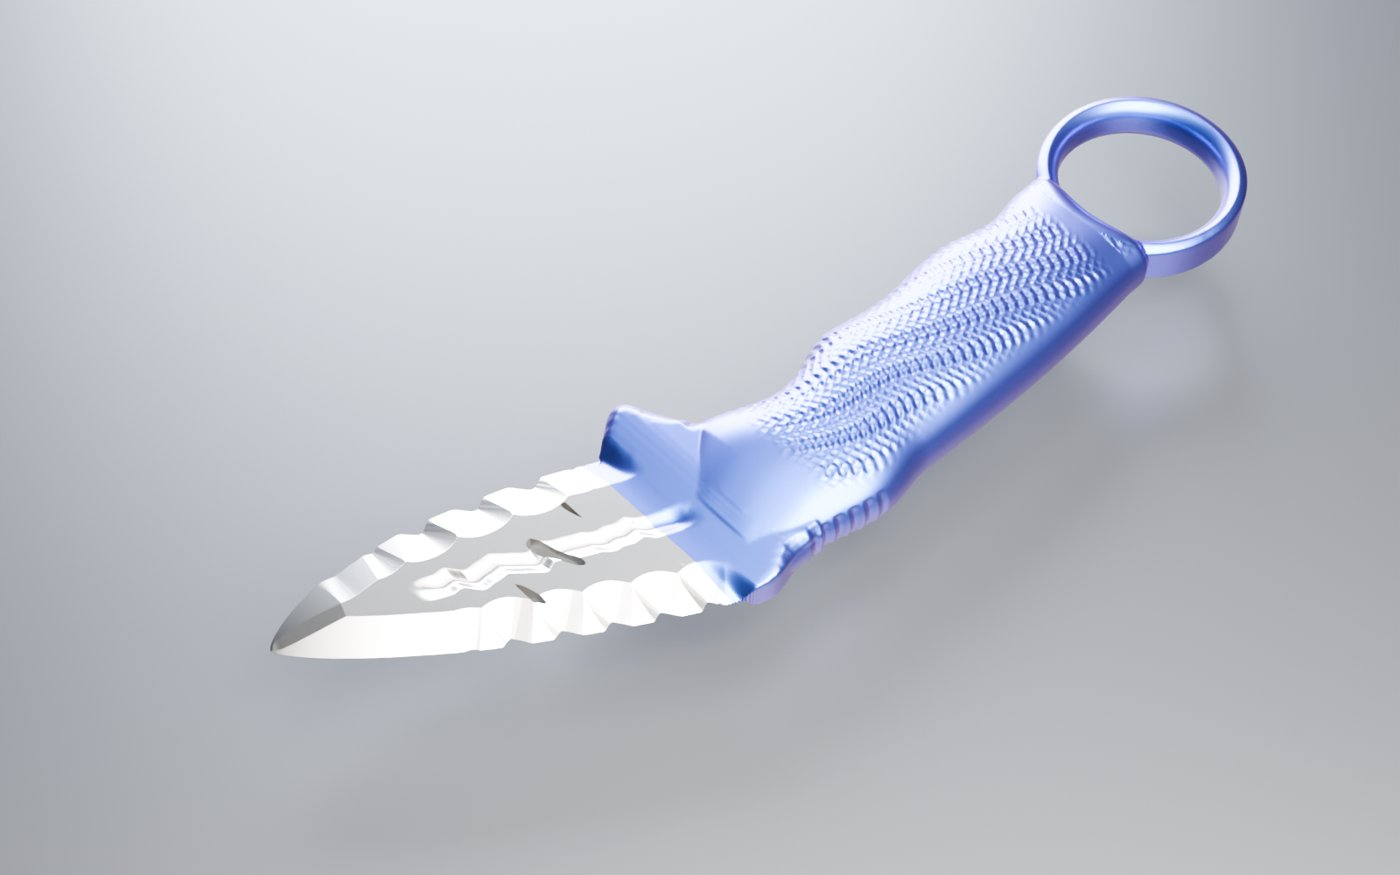
\includegraphics[width=0.49\textwidth]{hero.jpg}\hfill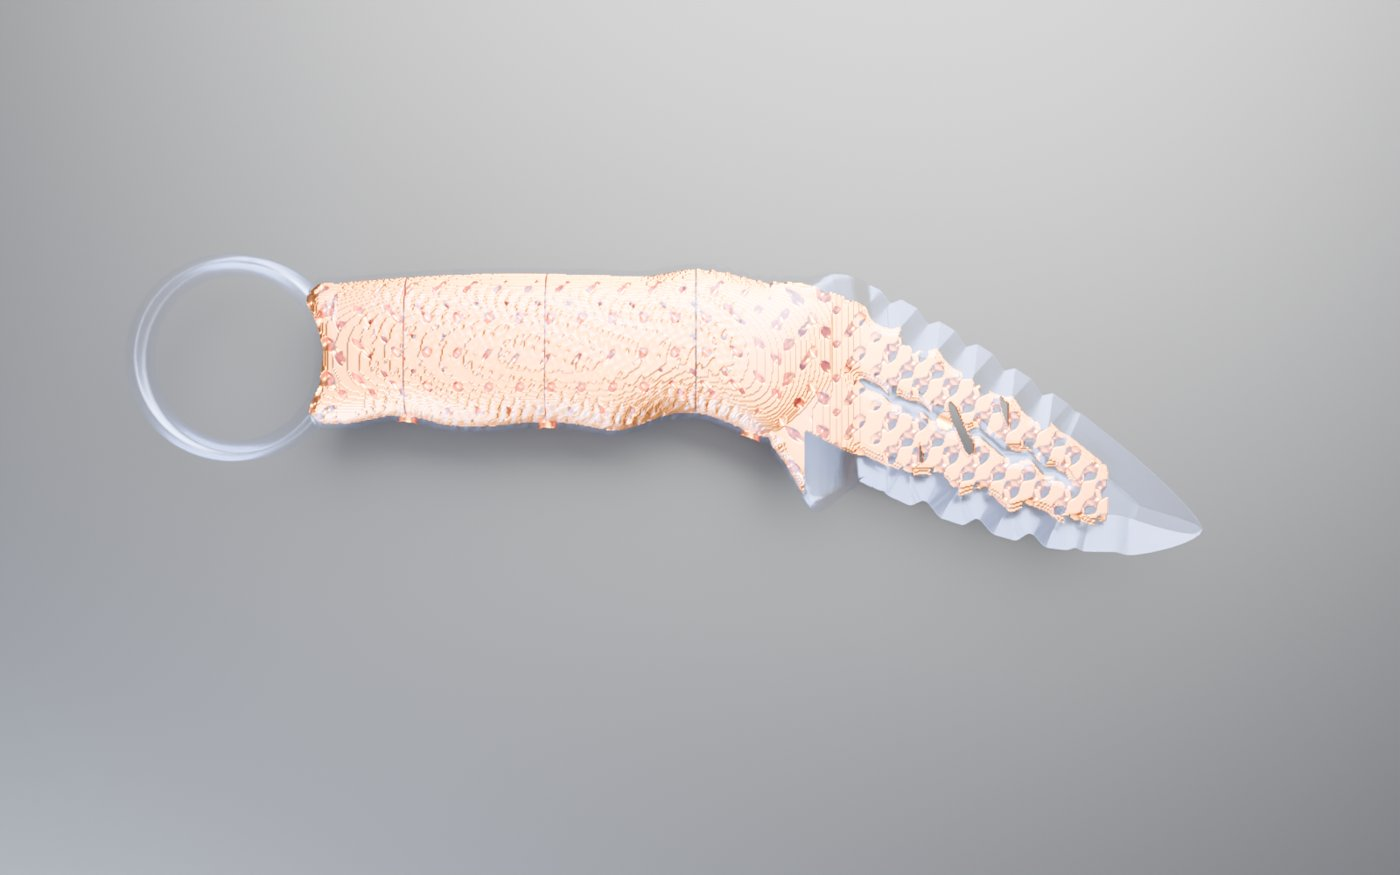
\includegraphics[width=0.49\textwidth]{xray.jpg}\\[3pt]
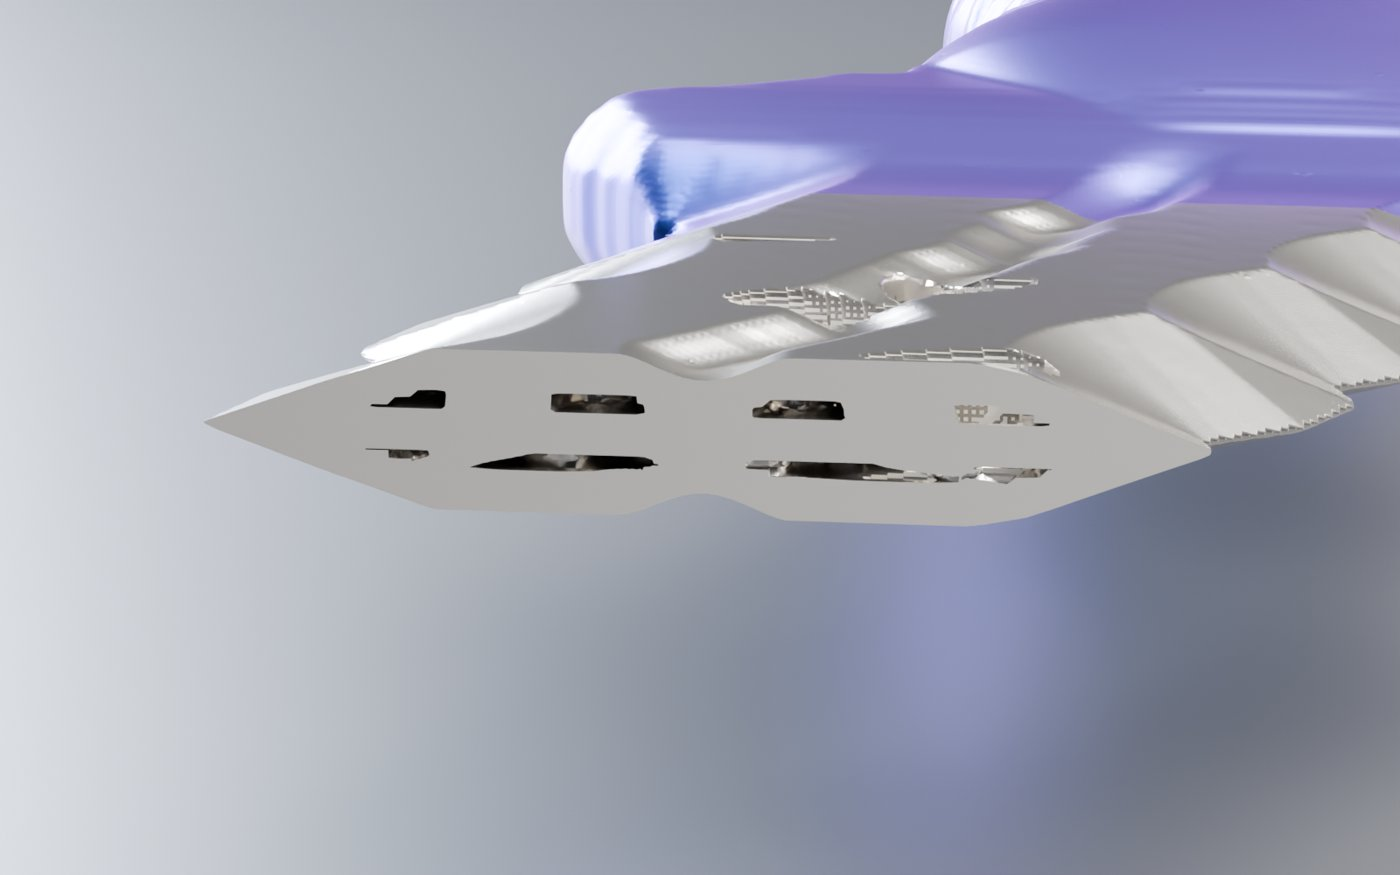
\includegraphics[width=0.32\textwidth]{cut_b.jpg}\hfill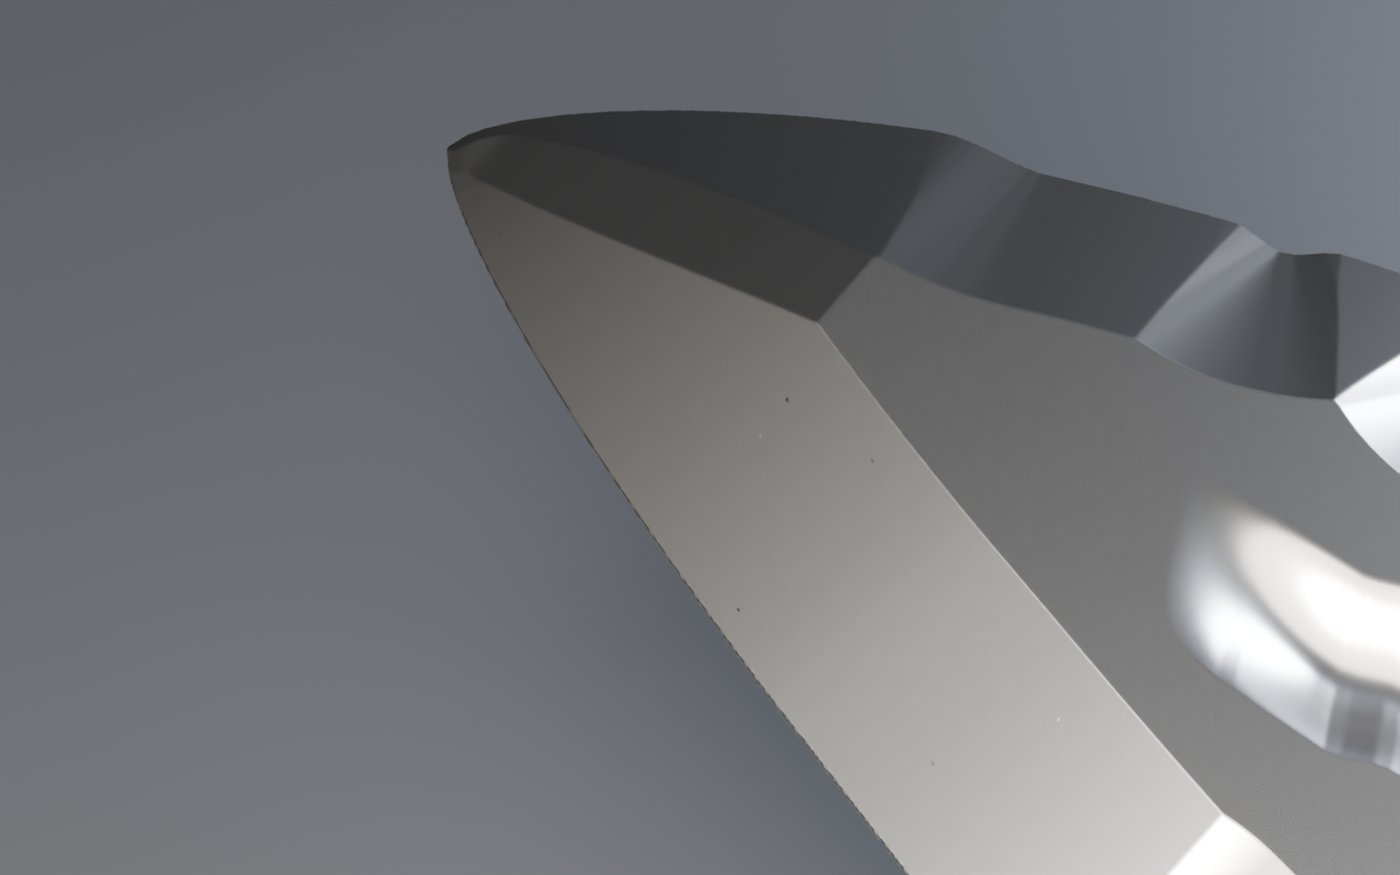
\includegraphics[width=0.32\textwidth]{tip.jpg}\hfill
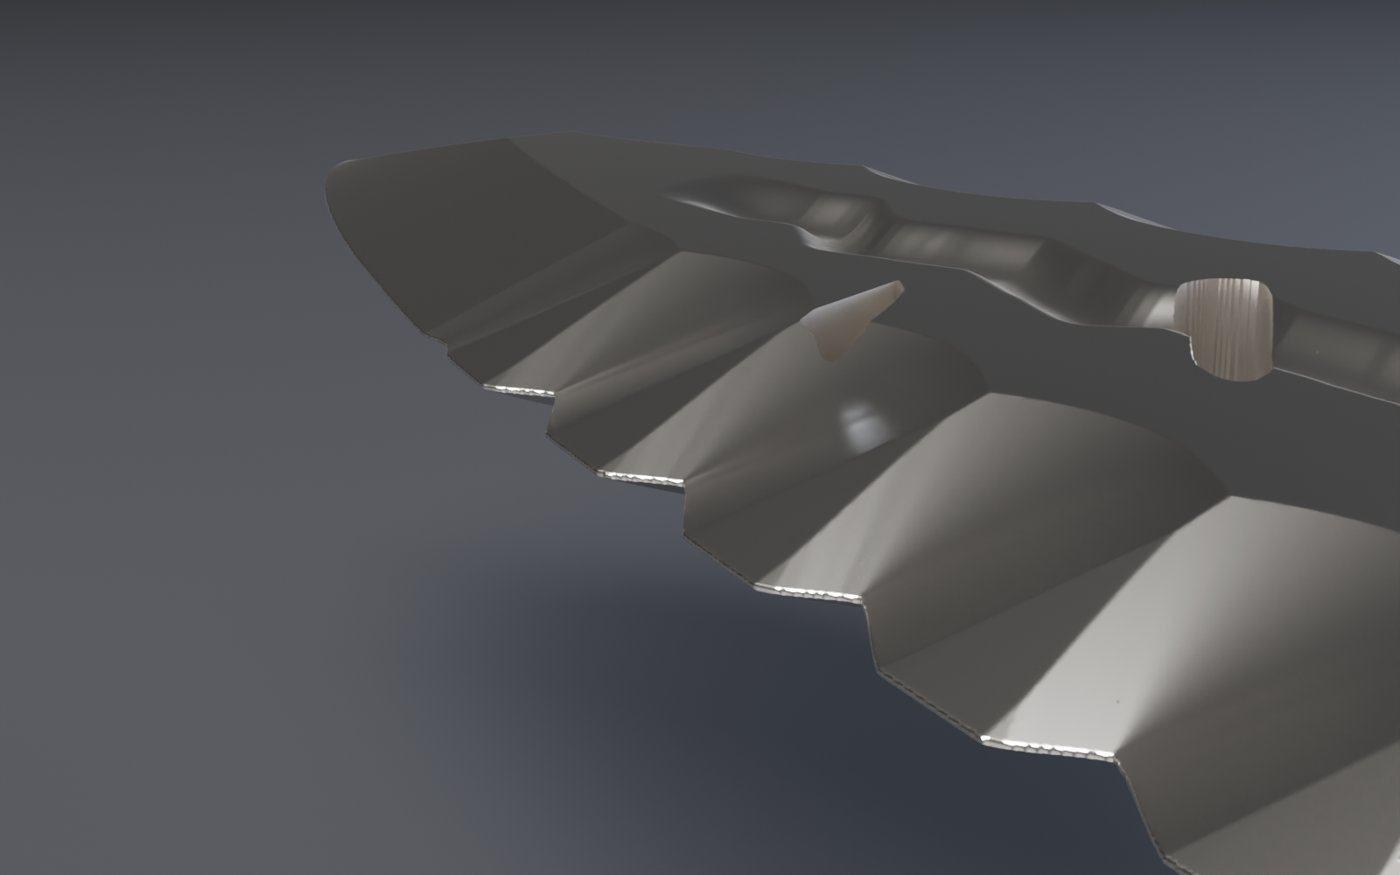
\includegraphics[width=0.32\textwidth]{edge_b.jpg}
\caption{\gDesign. Top: the knife, and an x-ray with every internal cavity in amber. Bottom: a section across the blade
30 mm from the point, the point, and the spine edge with its serrations. Cycles renders of the exported meshes; the blade
is meshed at 0.05 mm from the exact decoder law, the rest at 0.2 mm voxels.}\label{fig:hero}
\end{figure*}

\subsection{The best individual}
The best individual, \gDesign{} (genome hash \gGenomeSha), scores \gScore{} with a weighted base of \gBase{} and an
ergonomic multiplier of \gE. Its grip is \gLg{} mm long with a swell perimeter of \gSwellPerim{} mm and a height-to-width
ratio of \gHoT; the guard is \gGuardH{} mm high and the reach of the blade from the guard is \gReach{} mm. Its print mesh
weighs \gMassG{} g (Table~\ref{tab:mass} lists the four masses of this design). Fig.~\ref{fig:hero} shows it; Table~\ref{tab:best} lists its measurements.

\begin{table}[t]
\caption{Results for the best individual (platform of record; each model as labelled)}\label{tab:best}
\centering
\begin{tabular}{@{}lr@{}}
\toprule
Measure & Value \\
\midrule
Mass, print mesh (watertight, 0.2 mm) & \gMassG{} g \\
Edge A per-side angle, apex / bevel & \gEdgeAApexLo--\gEdgeAApexHi / \gEdgeABevelLo--\gEdgeABevelHi\textdegree \\
Edge B per-side angle, apex / bevel & \gEdgeBApexLo--\gEdgeBApexHi / \gEdgeBBevelLo--\gEdgeBBevelHi\textdegree \\
Grind ends from the point, A / B & \gEdgeATo{} / \gEdgeBTo{} mm \\
Unsharpened plunge, A / B & \gEdgeAPlunge{} / \gEdgeBPlunge{} mm \\
Serration depth, A / B & \gEdgeADepth{} / \gEdgeBDepth{} mm \\
Scallops, A / B & \gEdgeATeeth{} / \gEdgeBTeeth \\
Weakest tooth SF, A / B (teeth checked) & \gEdgeAToothSF{} / \gEdgeBToothSF{} (\gEdgeATeethChecked{} / \gEdgeBTeethChecked) \\
Solid tip SF (1.82 N$\cdot$m twist) & \gTipSF \\
Lateral capacity (search plate mesh) & \gLatN{} N \\
Grip SF, worst of four cases (formula) & \gGripSF \\
Human-max twist SF (search plate mesh) & \gHmTwist \\
Spine 3427 N SF (search plate mesh) & \gHmSpine \\
Ring bearing / back capacity & \gRingBear{} / \gRingBack{} N \\
Fatigue SF / yield-sequence ratio (as coded) & \gFat{} / \gSeq \\
Buckling factor $\lambda$ (analytic) & \gBuck \\
\bottomrule
\end{tabular}
\end{table}

\subsection{Diagnostics added in v3.0.3}\label{sec:diag}
Four diagnostics re-examine this design without changing its receipt or the ranking (\code{g3-diagnostics};
\code{evidence/g3/v\gRecord/diagnostics/}).
\begin{itemize}
\item \textbf{Yield sequence per load case.} The ratio in Table~\ref{tab:best} divides the grip's worst safety factor,
set by the spine load, by the blade's under the 260~N lateral load, so it mixes two load cases. Taken per case with the
voxel-FE grip factors, the ratios are \gSeqLat{} (lateral), \gSeqTwist{} (twist) and \gSeqSpine{} (spine); only the spine
case is below 1.2.
\item \textbf{Fatigue.} The coded fatigue stress divides the plate peak by the thin-wall knock-down \gJointK{} that the
allowable already carries. Applied once, the factor is \gFatCorr{} instead of \gFat.
\item \textbf{Solid tip.} The thickness raster fed to the TET10 model is filled at cell corners and read at cell
centres, a half-cell offset. With the offset removed, the production mesh gives \gTipRaster{} instead of \gTipSF. The
point is blunt in plan view: its included angle is \gTipAngleOne, \gTipAngleTwo{} and \gTipAngleThree\textdegree{} at
1, 2 and 3~mm from the point (\gTipWidthTwo~mm wide at 2~mm), which the thickness-only point gate does not measure.
\item \textbf{Plate model.} Refining the search's blade plate mesh to maximum element areas of \gPlateAreaA,
\gPlateAreaB, \gPlateAreaC{} and \gPlateAreaD~mm$^2$ gives lateral capacities of \gPlateLatA, \gPlateLatB, \gPlateLatC{}
and \gPlateLatD~N. The series does not converge, as a peak stress at sharp features does not, so the plate's lateral,
twist and spine values are values of the search model, not converged estimates.
\item \textbf{Mass.} Table~\ref{tab:mass} lists the four masses of the design. Scored at its print-mesh mass it would
score \gScoreAtMesh{} instead of \gScore. The grip holds \gZoneGripPct~\% of the printed mass, the blade
\gZoneBladePct~\% and the ring \gZoneRingPct~\%.
\end{itemize}

\begin{table}[t]
\caption{The four masses of the best individual}\label{tab:mass}
\centering
\begin{tabular}{@{}lr@{}}
\toprule
Definition & Mass (g) \\
\midrule
Search voxel count, $h = \gH$ mm & \gMassVoxelG \\
Ranking voxel count, $h = \gHRank$ mm (scored) & \gMassRankG \\
Print mesh, watertight, 0.2 mm (of record) & \gMassG \\
Upload mesh in \code{cad/} (coarser, under 50 MiB) & \gMassUploadG \\
\bottomrule
\end{tabular}
\end{table}

\begin{figure}[!t]
\centering
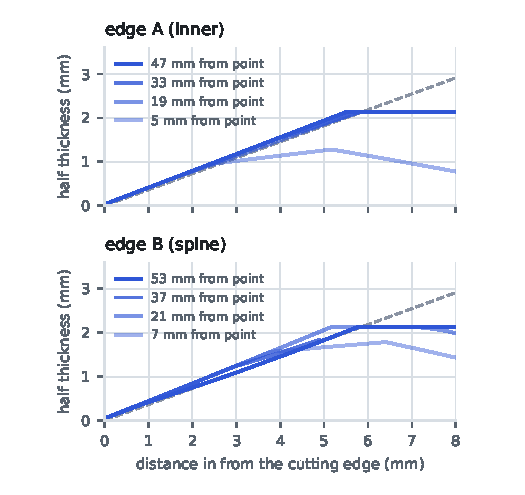
\includegraphics[width=\linewidth]{edge_sections.pdf}
\caption{Upper half of the blade section at four stations of each edge, true scale, against a 20\textdegree{} per-side
grind (dashed). Profiles stop where a lightening slot begins.}\label{fig:edges}
\end{figure}

\subsection{Edges and serrations}
Fig.~\ref{fig:edges} plots the blade section at four stations of each edge, measured along the true edge normal with the
exact decoder law. Every station of an edge lies on one line: edge A at \gEdgeAApexLo--\gEdgeAApexHi\textdegree{} per side
and edge B at \gEdgeBApexLo--\gEdgeBApexHi\textdegree, with no slope steeper than \gEdgeASteep\textdegree{} and
\gEdgeBSteep\textdegree{} within 2 mm of the edge. Both edges are serrated over the rear part of the blade, and the
grinds run on through the plain point region to \gEdgeATo{} and \gEdgeBTo{} mm from the point. Of the teeth between scallops (\gEdgeATeethChecked{} on edge A and \gEdgeBTeethChecked{} on edge B), the weakest has a
safety factor of \gToothMin{} under the \gToothSnag{} N snag and \gToothPry{} N pry, which \gToothReading{} of 1; the end
tooth of each span, bounded by a scallop on one side only, is not checked.
